    \section{Vista de Casos de Uso} \label{vistaCasosDeUso}
    En esta vista se describirá el sistema desde el punto de vista de los casos de uso. El sistema tiene 3 actores:

    \begin{itemize}
        \item \emph{Customer}: representa a una o varias estaciones de servicio. Solo tiene acceso a la información referente a las estaciones de servicio asignadas por el administrador del sistema. Es el tipo de usuario que más uso le dará al sistema.
        \item \emph{Staff}: representa a un distribuidor de combustible. Tiene acceso a la información de todas las estaciones de servicio del sistema.
        \item \emph{Admin}: administrador del sistema. Tiene acceso al \emph{back end} de Umbraco y puede gestionar (realizar las acciones CRUD) todas las entidades del sistema, incluyendo a los usuarios.
    \end{itemize}

    \subsection{Resumen de Casos de Uso}
    \newcounter{magicrownumbers}
    \newcommand\rownumber{\stepcounter{magicrownumbers}\arabic{magicrownumbers}}
    \begin{center}
        \begin{longtable}{ |c|c|c| }
            \hline
            \rowcolor{lightgray}
            ID Caso de Uso & Caso de Uso & Actor \\
            \hhline{===}
            \endhead

            \endfoot

            CU-\rownumber & Gestionar usuarios & Admin \\ \hline
            CU-\rownumber & Consultar lista de usuarios & Admin \\ \hline
            CU-\rownumber & Gestionar usuario (CRUD) & Admin \\ \hline
            CU-\rownumber & Asignar cliente/s a usuario & Admin \\ \hline
            CU-\rownumber & Remover cliente/s de usuario & Admin \\ \hline
            CU-\rownumber & Cambiar permisos de usuario & Admin \\ \hline

            CU-\rownumber & Gestionar contenido & Admin \\ \hline
            CU-\rownumber & Consultar lista de clientes & Admin \\ \hline
            CU-\rownumber & Gestionar cliente (CRUD) & Admin \\ \hline
            CU-\rownumber & Consultar lista de productos & Admin \\ \hline
            CU-\rownumber & Gestionar producto (CRUD) & Admin \\ \hline
            CU-\rownumber & Consultar lista de transportes & Admin \\ \hline
            CU-\rownumber & Gestionar transportes (CRUD) & Admin \\ \hline
            CU-\rownumber & Consultar lista de zonas & Admin \\ \hline
            CU-\rownumber & Gestionar zonas (CRUD) & Admin \\ \hline

            CU-\rownumber & Gestionar transacciones & Admin \\ \hline
            CU-\rownumber & Consultar lista de registros & Admin \\ \hline
            CU-\rownumber & Gestionar registro (CRUD) & Admin \\ \hline
            CU-\rownumber & Consultar lista de pedidos & Admin \\ \hline
            CU-\rownumber & Gestionar pedido (CRUD) & Admin \\ \hline
            CU-\rownumber & Consultar lista de detalles de pedidos & Admin \\ \hline
            CU-\rownumber & Gestionar detalle de pedido (CRUD) & Admin \\ \hline
            CU-\rownumber & Consultar lista de facturas & Admin \\ \hline
            CU-\rownumber & Gestionar factura (CRUD) & Admin \\ \hline
            CU-\rownumber & Consultar lista de cobros & Admin \\ \hline
            CU-\rownumber & Gestionar cobro (CRUD) & Admin \\ \hline
            CU-\rownumber & Consultar lista de detalles de cobros & Admin \\ \hline
            CU-\rownumber & Gestionar detalle de cobro (CRUD) & Admin \\ \hline

            CU-\rownumber & Iniciar sesión & Customer, Staff \\ \hline
            CU-\rownumber & Consultar lista de pedidos & Customer, Staff \\ \hline
            CU-\rownumber & Consultar pedido & Customer, Staff \\ \hline
            CU-\rownumber & Filtrar lista de pedidos & Customer, Staff \\ \hline
            CU-\rownumber & Exportar lista de pedidos & Customer, Staff \\ \hline
            CU-\rownumber & Crear pedido & Customer, Staff \\ \hline
            CU-\rownumber & Seleccionar cliente & Customer, Staff \\ \hline
            CU-\rownumber & Seleccionar fecha & Customer, Staff \\ \hline
            CU-\rownumber & Seleccionar turno  & Customer, Staff \\ \hline
            CU-\rownumber & Seleccionar transporte  & Customer, Staff \\ \hline
            CU-\rownumber & Seleccionar productos & Customer, Staff \\ \hline

            CU-\rownumber & Consultar lista de facturas & Customer, Staff \\ \hline

            CU-\rownumber & Consultar lista de clientes & Customer, Staff \\ \hline
            CU-\rownumber & Consultar cliente & Customer, Staff \\ \hline
            CU-\rownumber & Consultar pedidos de cliente & Customer, Staff \\ \hline

            CU-\rownumber & Consultar lista de transportes & Customer, Staff \\ \hline

            CU-\rownumber & Importar lista de transportes & Customer, Staff \\ \hline

            CU-\rownumber & Consultar lista de zonas & Customer, Staff \\ \hline

            CU-\rownumber & Importar lista de zonas & Customer, Staff \\ \hline

        \end{longtable}
    \end{center}

    \subsection{Diagrama de Casos de Uso}
    Se separaron los casos de uso en varios diagramas para facilitar la lectura.

    \begin{figure}[H]
        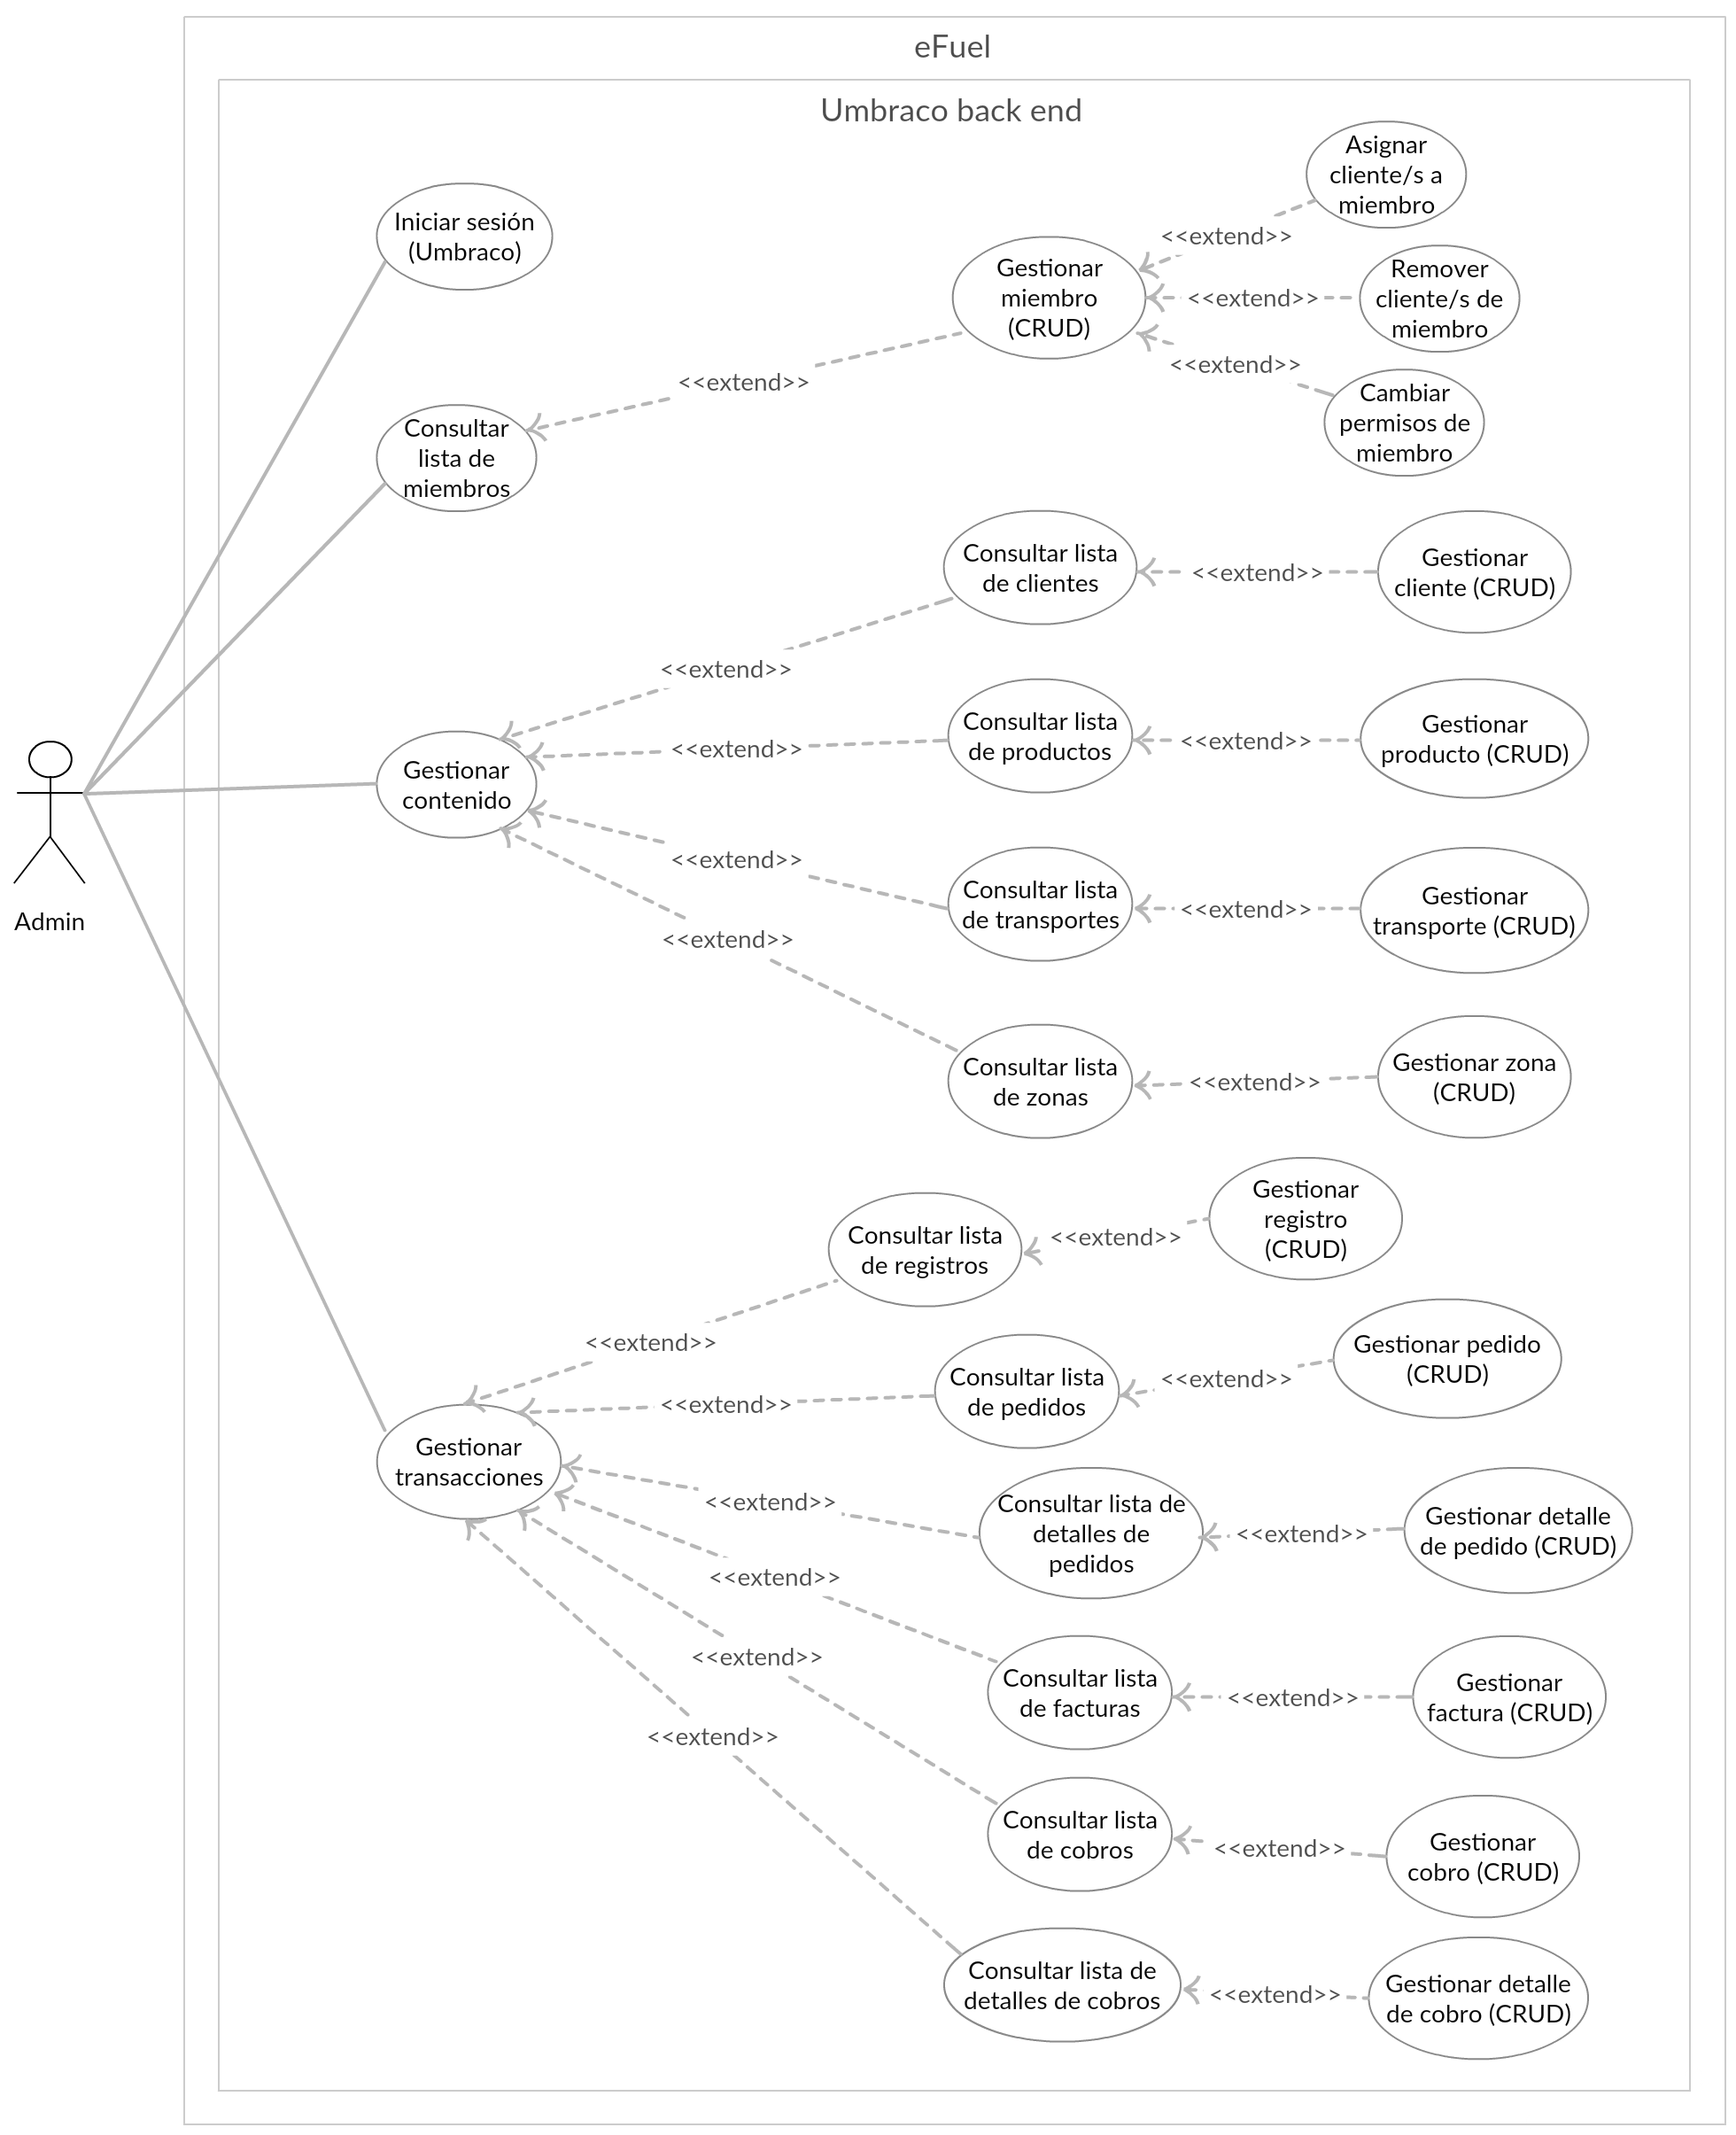
\includegraphics[width=\textwidth]{cu_admin.png}
        \centering
    \end{figure}

    \begin{figure}[H]
        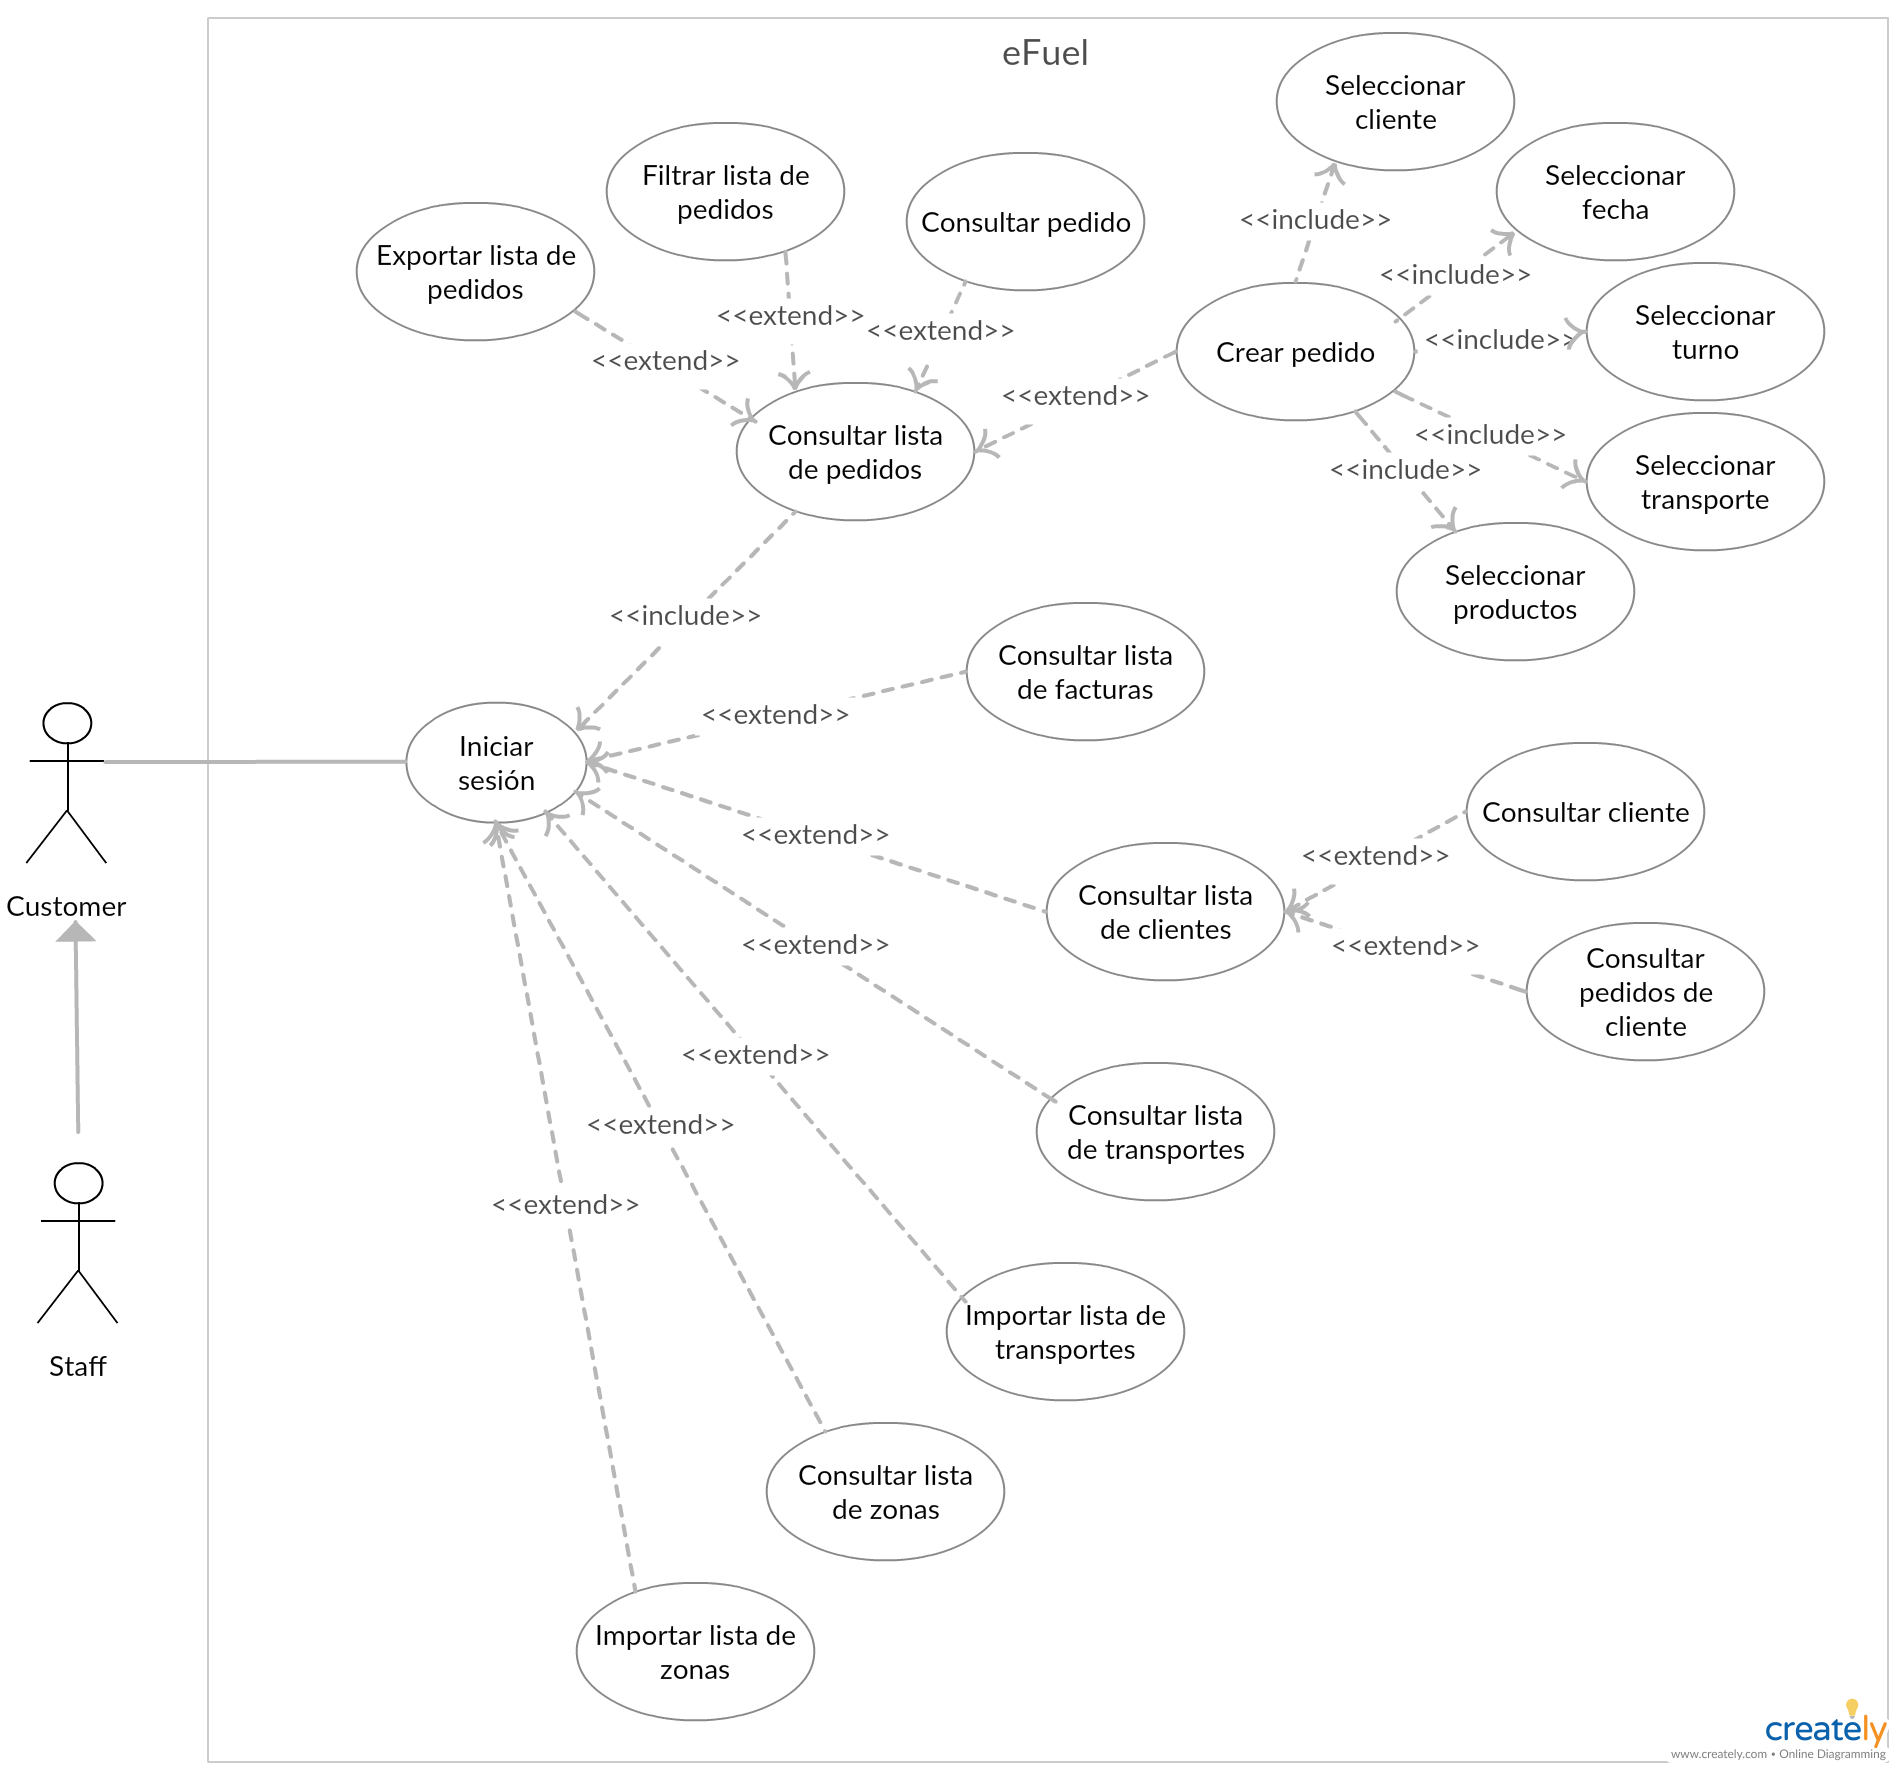
\includegraphics[width=\textwidth]{cu_customer_staff.png}
        \centering
    \end{figure}

    \subsection{Especificaciones de Casos de Uso}
    A continuación las narrativas de los casos de uso:



